\documentclass[aspectratio=149]{beamer}
\usepackage[english]{babel}
\usepackage{uep_kie_ms}
\usepackage{makecell}

\setbeamertemplate{footline}[text line]{

\includegraphics[height=0.7cm]{logo_uep}
\hspace*{8cm}~%

\includegraphics[height=0.7cm]{logo_ncbr_en}
}

\author{Marcin~Sawiński}
\date{2023-10-25}
\institute{Poznań University of Economics and Business} 
\title{Finetuning Llama 2 with PEFT QLoRa method for detecting Check-worthy Claims}
\subtitle{Follow-up on CheckThat! Lab at CLEF 2023}

\begin{document}

\begin{frame}
\begin{figure}
% 
\includegraphics[height=1cm]{logo_clef}
% \hspace*{0.5cm}~%

\includegraphics[height=1cm]{logo_openfact}
\hspace*{0.5cm}~%

\includegraphics[height=1cm]{logo_infos.png}
\hspace*{0.5cm}~%

\includegraphics[height=1cm]{logo_godlo_flaga}
\end{figure}
\fontsize{7pt}{7pt}\selectfont
OpenFact -- AI tools for verification of veracity of information sources and fake news detection.\\ Financed by National Center for Research and Development in Poland (INFOSTRATEG-I/0035/2021-00).

\titlepage
\end{frame}
%%%%%%%%%%%%%%%%%%%%%%%%%FRAME%%%%%%%%%%%%%%%%%%%%%%%%%
\begin{frame}{Experiments}
\begin{itemize}
  \item Setup cloud infrastrcuture for running custom Llama 2 Models
  \item Prepare training and infernece pipeliens for 7B, 13 B and 70B model variants.
  \item Use 3 datasets variants (full, 2:1 and 1:1)
\end{itemize}
\end{frame}

%%%%%%%%%%%%%%%%%%%%%%%%%FRAME%%%%%%%%%%%%%%%%%%%%%%%%%
\begin{frame}{Curating dataset - fewer, better data}
\begin{itemize}
  \item Original train data set size - 16821
  \item Curated train data set size 2:1 NCS/CS - 7692
  \item Downsampled train data set size 1:1 NCS/CS (randomly picked)

\end{itemize}

\begin{figure}[h]
    \centering
    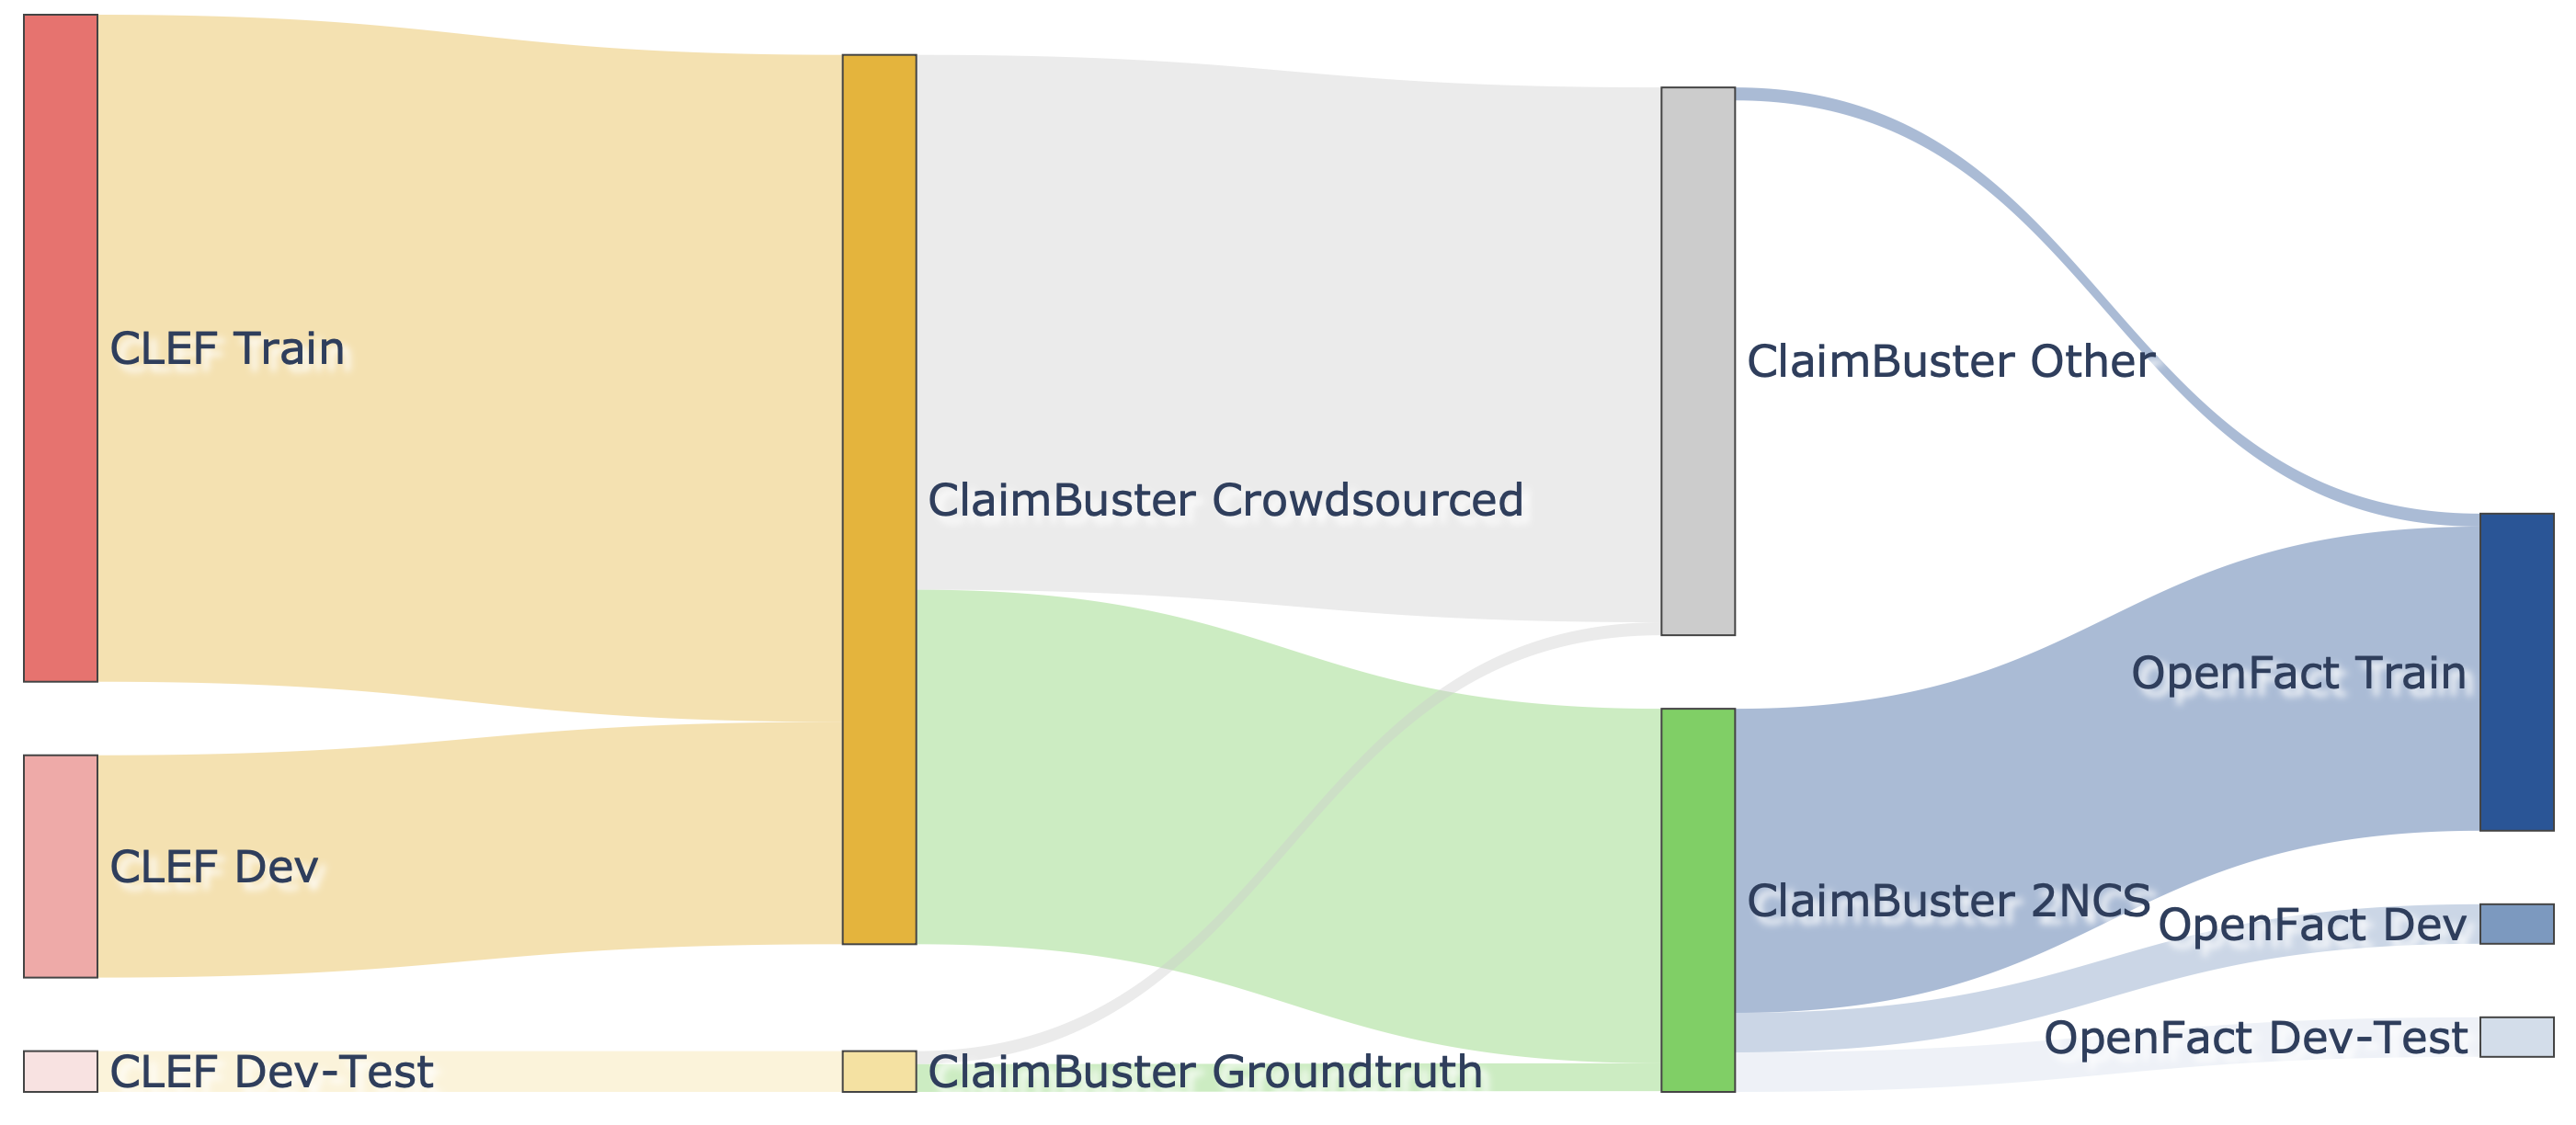
\includegraphics[width=10cm]{./sank}
\caption{Reshuffling of 2:1 dataset}
\end{figure}
\end{frame}
%%%%%%%%%%%%%%%%%%%%%%%%%FRAME%%%%%%%%%%%%%%%%%%%%%%%%%
\begin{frame}{Stating point - Perspectives for future work}
  \begin{itemize}
\item More resources / bigger models / smaller models
\item Examine dataset curation impact
\item Chain-of-Thought and beyond
\end{itemize}

\end{frame}
%%%%%%%%%%%%%%%%%%%%%%%%%FRAME%%%%%%%%%%%%%%%%%%%%%%%%%
\begin{frame}{Downsampled datasets further increased detecion f1 score}
\begin{figure}[h]
\centering
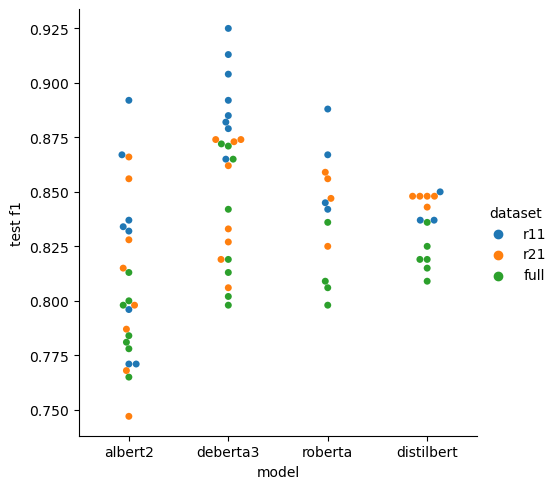
\includegraphics[width=8cm]{./f1}
\end{figure}
\end{frame}
%%%%%%%%%%%%%%%%%%%%%%%%%FRAME%%%%%%%%%%%%%%%%%%%%%%%%%
\begin{frame}{Fine-tuning Llama 2}
Llama 2 is pretreained model from Meta\footnote{https://ai.meta.com/llama/}, trained on corpus of 2 Trillion tokens. Further finetuning was performed usign 1'000'000 human annotations.
Inference infra chosen in GCP:
\begin{itemize}
  \item abc
%   \item 7B model - Machine type: g2-standard-8 Accelerator : NVIDIA_L4 x 1
%   \item 13B model - Machine type: g2-standard-24 Accelerator : NVIDIA_L4 x 2
%   \item 70B model - Machine type: g2-standard-96 Accelerator : NVIDIA_L4 x 8
\end{itemize}
\end{frame}
%%%%%%%%%%%%%%%%%%%%%%%%%FRAME%%%%%%%%%%%%%%%%%%%%%%%%%
\begin{frame}{Hyperparamters}
\centering
\begin{table}
\label{tab:finetuning-hyperparams}
\begin{tabular}{lc}
        \toprule
        \textbf{Hyperparameter}        & \textbf{Value} \\
        \midrule
        Batch size                     & 8              \\ 
        Learning rate multiplier       & 0.1            \\ 
        Epochs                         & 4              \\ 
        Prompt loss weight             & 0.01           \\ 
        Compute classification metrics & True           \\ 
\bottomrule
    \end{tabular}
\caption{Hyperparameters used for fine-tuning GPT-3 models}
\end{table}
\end{frame}
%%%%%%%%%%%%%%%%%%%%%%%%%FRAME%%%%%%%%%%%%%%%%%%%%%%%%%
% \begin{frame}{abc}
% %   `device_map` requires Accelerate: `pip install accelerate`


% %   Failed to import transformers.trainer because of the following error (look up to see its traceback):
% % [Errno 13] Permission denied: '/root/google_vm_config.lock'
% % PermissionError: [Errno 13] Permission denied: '/root/google_vm_config.lock'
% % /usr/bin/env /opt/conda/bin/python cp_train_template_llama.py

% % https://github.com/TimDettmers/bitsandbytes/issues/620
% % nano cd /opt/conda/lib/python3.10/site-packages/bitsandbytes/cuda_setup/env_vars.py

% % GOOGLE_VM_CONFIG_LOCK_FILE

% % to the set ignorable inside def to_be_ignored 
% \end{frame}
%%%%%%%%%%%%%%%%%%%%%%%%%FRAME%%%%%%%%%%%%%%%%%%%%%%%%%
\begin{frame}{Experiments results}
\fontsize{9pt}{10pt}\selectfont
\begin{table}[!htb]
    \centering
%    \caption{The results obtained by the GPT and BERT models}
    \label{tab:results}
    \begin{tabular}{lrrrr}
        \toprule
        Model                              & F1    & precision & recall & accuracy \\
        \midrule
        GPT-3 curie fine-tuned curated     & 0.898 & 0.948     & 0.852  & 0.934    \\
        DeBERTa v3 base fine-tuned         & 0.894 & 0.978     & 0.824  & 0.934    \\
        GPT-3 davinci fine-tuned curated   & 0.876 & 0.946     & 0.815  & 0.921    \\
        RoBERTa base fine-tuned            & 0.862 & 0.966     & 0.778  & 0.915    \\
        \makecell[l]{RoBERTa base fine-tuned with custom                           \\optimizer layer-wise learning rate decay} & 0.860 &      0.976 &   0.769 &     0.915 \\
        \makecell[l]{LightGBM ensemble of all BERT-based                           \\models and additional embeddings} & 0.854 &      0.976 &   0.759 &     0.912 \\
        ELECTRA fine-tuned                 & 0.851 & 0.954     & 0.769  & 0.909    \\
        AlBERT large v2 fine-tuned         & 0.848 & 0.976     & 0.750  & 0.909    \\
        DistilBERT base uncased fine-tuned & 0.827 & 0.952     & 0.731  & 0.896    \\
        GPT-3 curie fine-tuned random      & 0.826 & 1.000     & 0.704  & 0.899    \\
        GPT neo 125M fine-tuned            & 0.800 & 0.961     & 0.685  & 0.884    \\
        GPT-4 few-shot learning            & 0.788 & 0.867     & 0.722  & 0.868    \\
        GPT-4 zero-shot learning           & 0.778 & 0.710     & 0.861  & 0.833    \\
        GPT-4 Chain-of-Thought             & 0.722 & 0.574     & 0.972  & 0.745    \\
        \bottomrule
    \end{tabular}

\end{table}
\end{frame}


%%%%%%%%%%%%%%%%%%%%%%%%%FRAME%%%%%%%%%%%%%%%%%%%%%%%%%
\begin{frame}{Experiments results on curated dataset}
\fontsize{9pt}{10pt}\selectfont
\begin{table}[!htb]
    \centering
%    \caption{The results obtained by the GPT and BERT models}
    \label{tab:results2}
\begin{tabular}{lrrrr}
\toprule
                        Model &    f1 &  precision &  recall &  accuracy \\
\midrule
  GPT-3 curie fine-tuned curated & 0.898 &      0.948 &   0.852 &     0.934 \\
            RoBERTa base curated & 0.896 &      0.968 &   0.833 &     0.934 \\
      DeBERTa v3 base fine-tuned & 0.894 &      0.978 &   0.824 &     0.934 \\
GPT-3 davinci fine-tuned curated & 0.876 &      0.946 &   0.815 &     0.921 \\
         RoBERTa base fine-tuned & 0.862 &      0.966 &   0.778 &     0.915 \\
   GPT-3 curie fine-tuned random & 0.826 &      1.000 &   0.704 &     0.899 \\
         DeBERTa v3 base curated & 0.818 &      0.900 &   0.750 &     0.887 \\
\bottomrule
\end{tabular}
\end{table}

\end{frame}
\end{document}


